\section{The LHC accelerator and the CMS experiment}\label{sec:lhc-cms}
\subsection{The Large Hadron Collider}\label{subsec:lhc}

The Large Hadron Collider (LHC) at the European Organisation for Nuclear Research (CERN), in Geneva, Switzerland is the highest-energy particle accelerator constructed to date. 
It is designed to operate at a centre of mass (CoM) energy of 14\TeV, through two 7\TeV proton beams travelling in 2808 bunches of up to $1.15 \times 10^{11}$ protons at a collision rate of 25\nsm which corresponds to a design luminosity of $10^{34}\percms$. 
The LHC can also operate in a heavy-ion mode, where lead ions are collided at 2.76\TeV per nucleon usually for one month a year~\cite{Bayatian:2006zz}.

Unlike matter-antimatter colliders, such as the Large Electron-Positron and Tevatron colliders, where the entirety of the centre of mass energy is available,  ... Advantage 

The beams collide at four interaction points around the LHC, with one of the four major experiments being based at each of them. 
The experiments are: A Toroidal LHC Apparatus (ATLAS) and the Compact Muon Solenoid (CMS) detectors, which are the two multi-purpose experiments; the Large Hadron Collider beauty (LHCb) is an experiment which specialises in b-physics and; A Large Ion Collider Experiment (ALICE), as the name suggests, specialises in heavy ion physics~\cite{Bruning:782076}.

Three smaller experiments are situated close to one of the four main experiments and use the same collision points.
Both the TOTal Elastic and diffractive cross section Measurement (TOTEM) and LHC-forward (LHCf) experiments study diffractive physics in the very-forward regions of collisions at the CMS and ATLAS experiments' collision points respectively.
Monopole and Exotics Detector At the LHC (MoEDAL) shares the LHCb experiment's cavern and performs direct searches for magnetic monopoles and highly ionising stable and pseudo-stable massive particles.

\subsubsection{Motivation}
The core motivations behind the LHC are to shed light on the nature of the electroweak symmetry breaking, which the Higgs was presumed and found to be responsible, and to probe the consistency of the SM above the \TeV level through precision measurements of SM parameters and the Higgs mechanism.
Alternative theories to the SM, such as SUSY theories, additional dimensions or new fundamental forces and particles are expected to emerge at and above the TeV level, giving the potential to ascertain whether these theories have any basis beyond mere conjecture.
%%% How this impacted experimental design choices
Measurements of the Higgs boson, precision measurements of SM parameters, and BSM physics (???) require a high interaction rate, which is ascertained through a high beam luminosity, due to their low production production probabilities in contrast to 

%Naturally the performance goals of the LHC machine were driven by the physics

The primary motivation behind operating the LHC in a heavy-ion mode is to search for evidence of the plasma of quarks and gluons, which is made possible through the resultant production of QCD matter under extreme temperature, density and low momentum fractions of partons~\cite{Baur:687318}.

\subsubsection{Accelerator Complex}
When operating in proton-proton mode, the preparation of the LHC beams starts at Linear accelerator 2 (Linac2). 
Protons from a hydrogen gas source are accelerated to 50\MeV and are injected into the Proton Synchrotron Booster which accelerates the protons to 1.4\GeV before injection into the Proton Synchrotron (PS). 
In the PS, the protons are accelerated to 26\GeV and are injected into the Super Proton Synchrotron (SPS) where they are accelerated to 450\GeV before finally entering the LHC~\ref{fig:cern-accelerator-complex}. 
When operating with lead ions, Linear accelerator 3 (Linac3) is used to initially accelerate the ions before injecting them into the Proton Synchrotron Booster, before the ions use the same accelerators as the protons do to prepare them for use in the LHC\~cite{Bruning:782076}. 

The LHC beam requires 1232 dipole magnets to bend the beam along its circular path and 392 quadrupole magnets to focus the beams, with each magnet producing a 8.3T field whilst operating at 1.9K.
Sixteen Radio Frequency (RF) cavities (eight per beam) are used to accelerate the beams up to their designed operational energies of 7\TeV over the course of circa twenty minutes. 
Each cavity operates at frequency of 400\MHz, at a temperature of 4.5K, delivering a maximum of 2 MV. 
The charged particles which pass through the cavities are accelerated by the energy imparted by the resonant electromagnetic field. 
If a charged particle arrives out of synchronisation with the operational frequency, such particles are either accelerated or decelerated so that they stay close to the energy of the ideal particle. 
This results in the charged particles being grouped into bunches before magnets near each of the four interaction points bend the beams so that they collide in the heart of the four main detectors.
A more detailed description of the LHC accelerator chain at CERN can be found in~\cite{Schindl:397574}. 

\begin{figure}[htbp]
\begin{center}
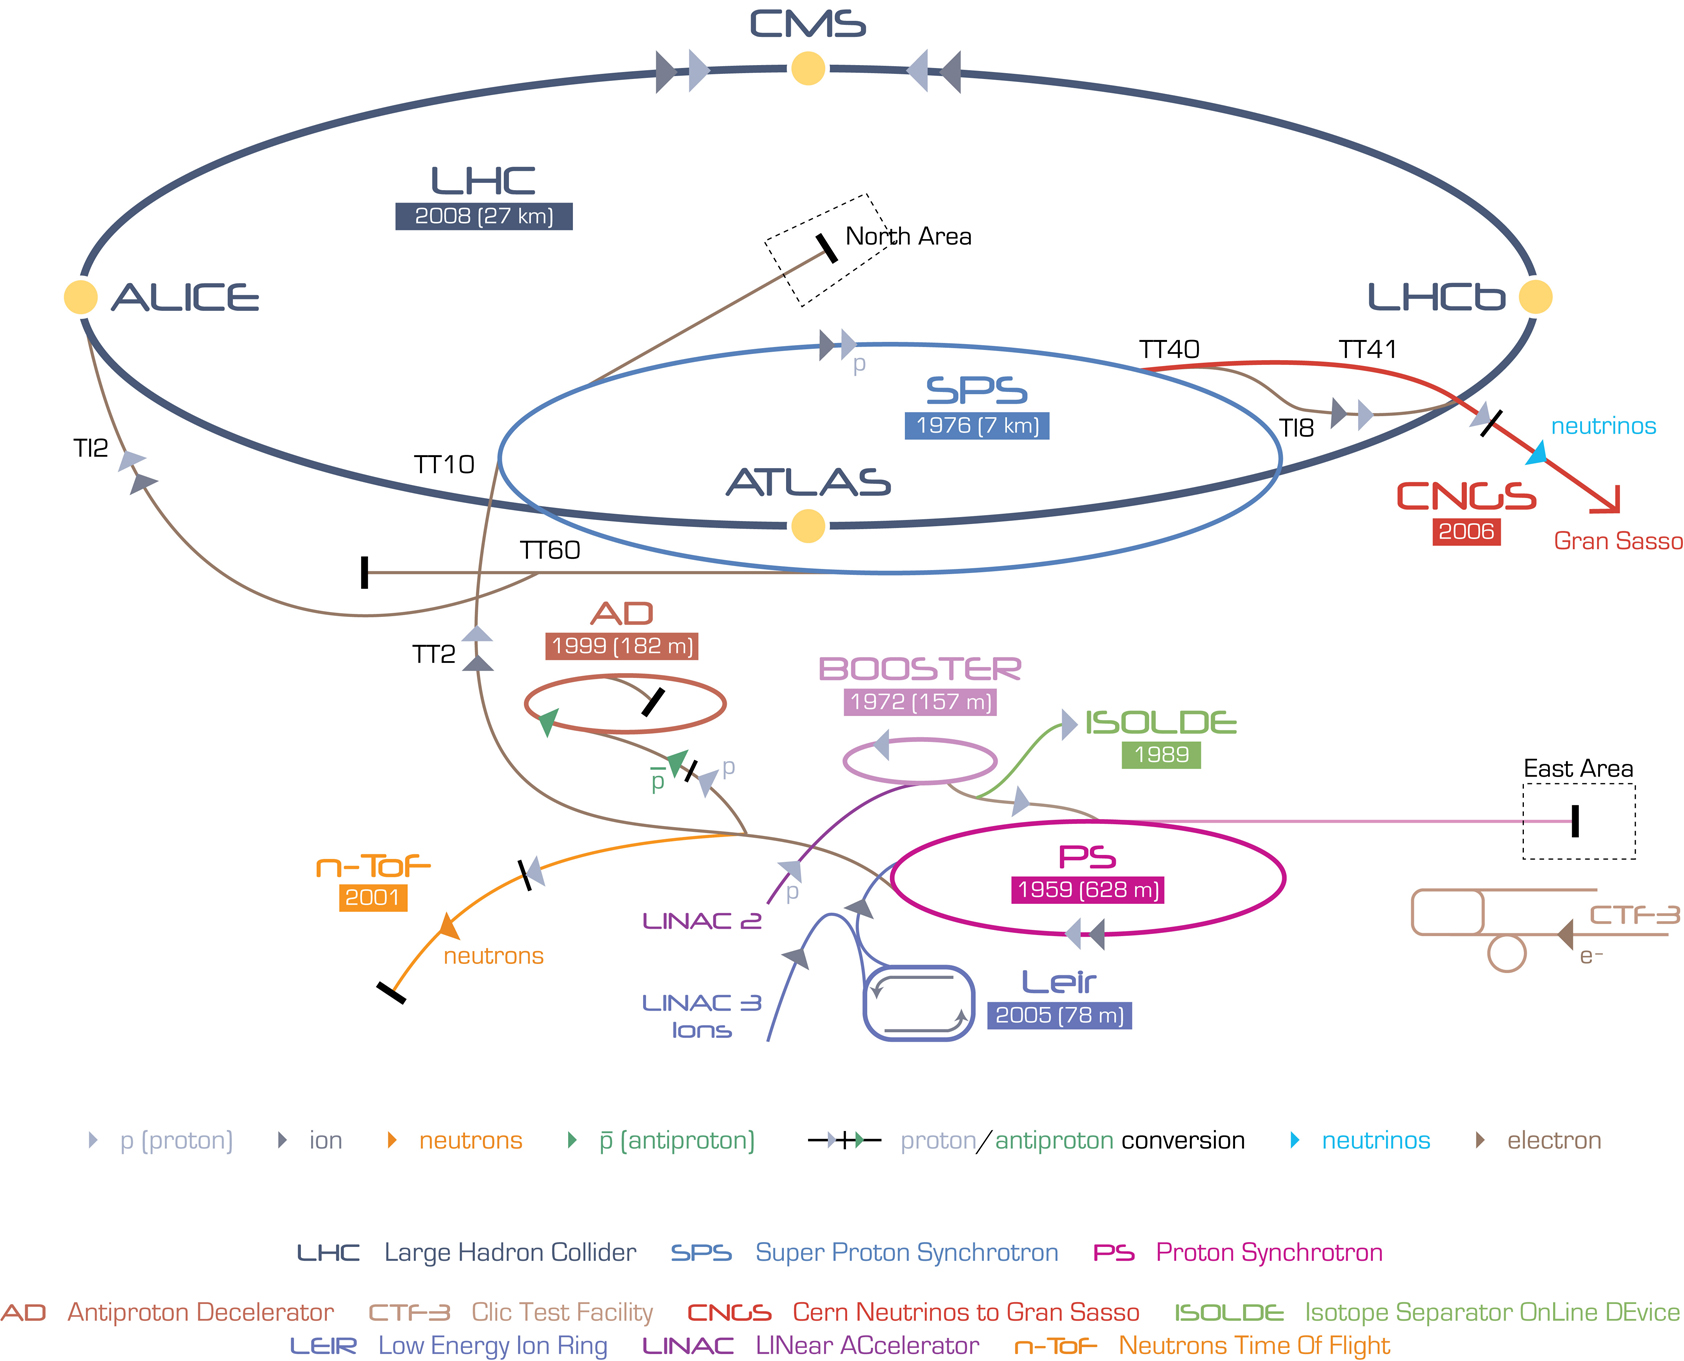
\includegraphics[width=0.97\textwidth]{figs/lhc/Cern-Accelerator-Complex.jpg}
\caption{CERN complex, including the various linear accelerators, synchrotrons, LHC, LHC detectors and other aspects of the complex.}
\label{fig:cern-accelerator-complex}
\end{center}
\end{figure}

\subsection{The Compact Muon Solenoid}\label{subsec:cms}

\subsubsection{Overview}
The Compact Muon Solenoid (CMS) is a large, general purpose, hermetic particle detector designed to investigate a wide range of physics phenomena and the smaller of the two multi-purpose experiments operating at the LHC at CERN. 

The design of the detector was motivated by the planned goals of the LHC's physics program. 


resulting in the distinguishing features of a high-field strength superconducting solenoid which fully encompasses the 
...


The CMS detector covers the rapidity range $\eta < 3$ at full resolution and covers an extended range $\eta < 5$ with the bending power being provided by a 13m long, 6m inner diameter, 4T superconducting solenoid.


The need for such a magnet comes from the requirement to precisely measure the momentum of high-energy charged particles, for high momentum charged particles spend less time passing through magnetic fields, resulting in a less curved trajectory.
The more powerful the magnet, the more precisely high-energy charged particles can be measured due to their greater displacement\cite{oldcms}.

Moving away from the centre of the detector and the particle beam, CMS consists of the inner tracking system (a pixel tracker and a silicon microstrip tracker), an electromagnetic calorimeter (ECAL), a hadronic calorimeter (HCAL), a 4T superconducting solenoid, an outer calorimeter (HO), and the muon chambers.
There is also a pair of very-forward calorimeters (HF) in the extended rapidity region\cite{oldcms}.

\begin{figure}[htbp]
\begin{center}
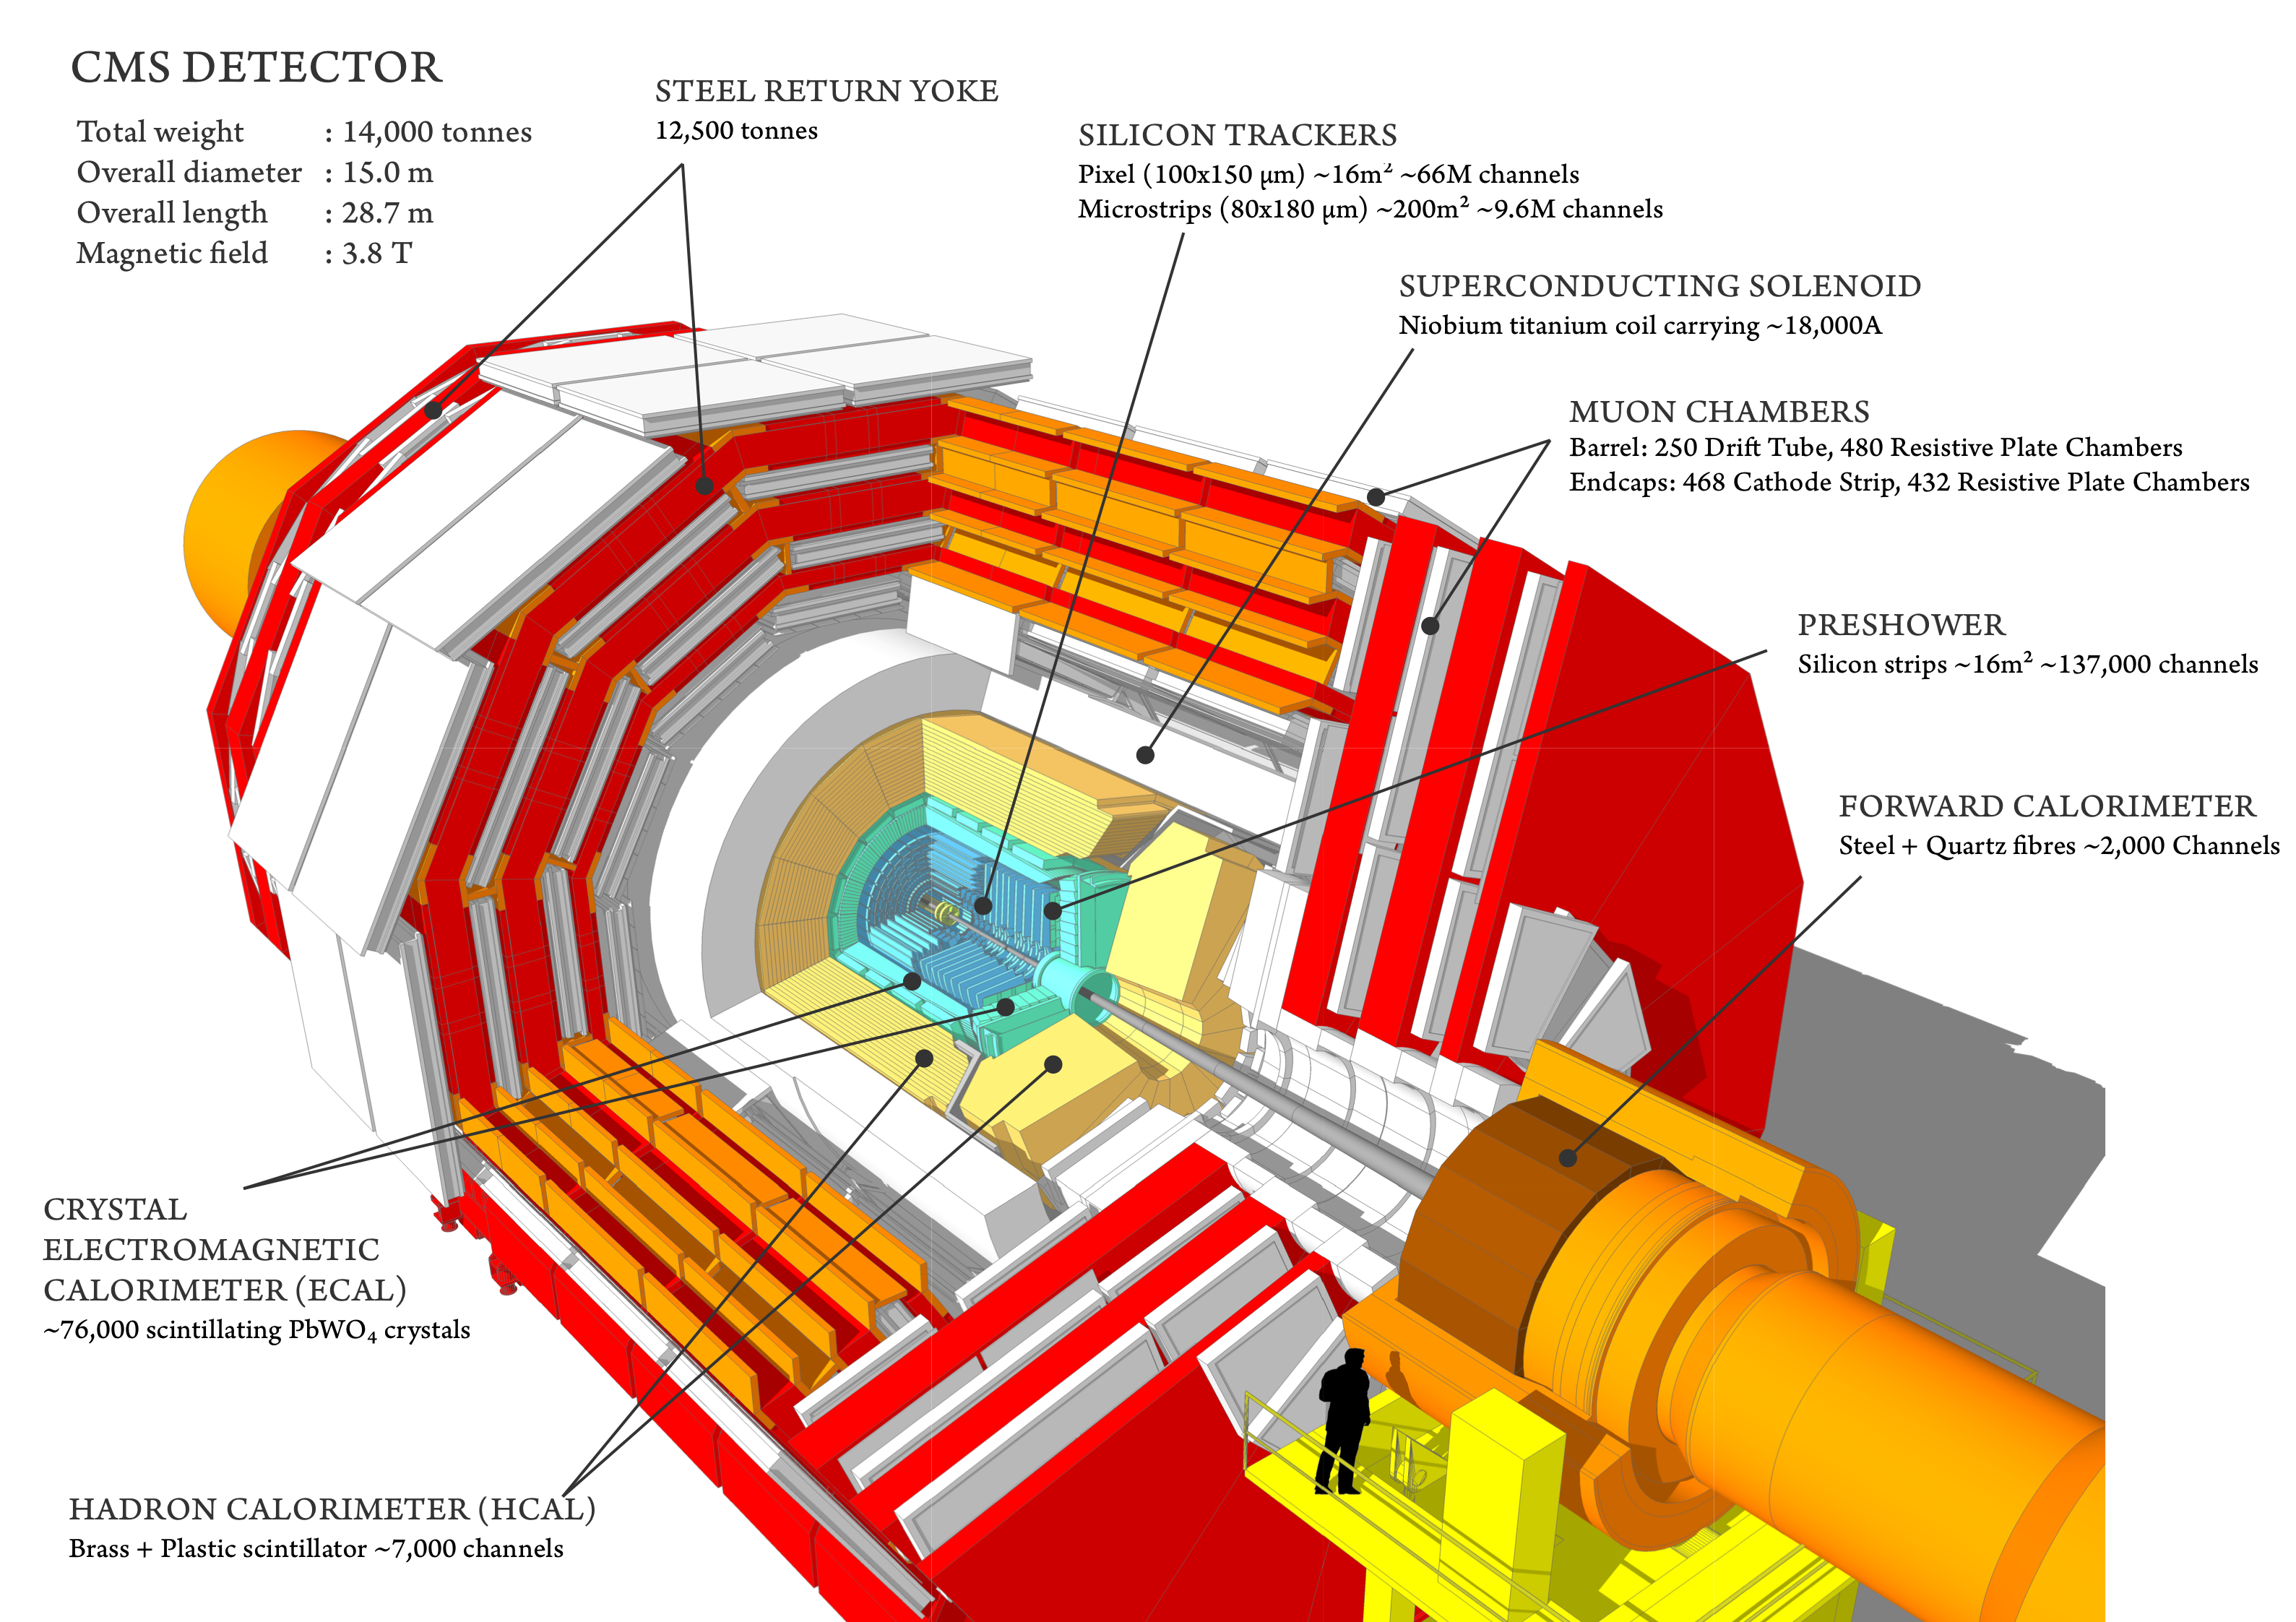
\includegraphics[width=0.97\textwidth]{figs/cms/cms_120918_03.png}
\caption{Cutaway diagram of CMS’s layers, illustrating its onion-like nature and the location of the detecting technologies within.}
\label{fig:cern-accelerator-complex}
\end{center}
\end{figure}

\begin{figure}[htbp]
\begin{center}
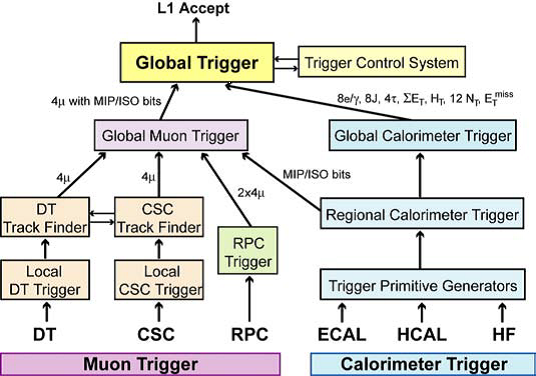
\includegraphics[width=0.97\textwidth]{figs/cms/trigger.png}
\caption{L-1 Trigger Architecture. Both muon and calorimeter triggers search for candidates locally before creating coarser datasets by passing on the most promising candidates to a higher level, and so on until the Global Trigger makes a final decision. However, unlike the Calorimeter Trigger, which looks at all the calorimeter systems concurrently, the Muon Trigger locally triggers on each of its detector technologies separately before submitting them to the Global Muon Trigger (with input from the Regional Calorimeter Trigger) before passing on fitted candidates to the Global Trigger.}
\label{fig:trigger}
\end{center}
\end{figure}

\subsubsection{Tracker}
The tracker, surrounding the interaction point, is designed to provide efficient precision trajectory measurements of charged particles emerging from collisions and precise reconstruction of secondary vertices over $\eta < 2.5$, whilst operating in a harsh radiation environment .
The tracker is composed of silicon, in order to limit charged particles interacting with the tracker (i.e. scattering, producing Bremsstrahlung), whilst providing the desired accuracy in track reconstruction\cite{oldcms}.

Measuring 5.8m 

%%Phase 1
During the 2016/2017 End of Year Technical Stop, 
\subsubsection{Electromagnetic Calorimeter}
The ECAL measures the energies of electrons and fermions through the scintillations they cause, which are proportional to their energy, as they pass through it.
The very dense lead tungstate crystals only emit a small amount of light (which has to be amplified), the light they do emit is well defined, short, and fast, resulting in precise data with very little latency\cite{oldcms}. 

\subsubsection{Hadronic Calorimeter}
The HCAL, comprised of brass/steel absorber plates interspersed with plastic scintillators, measures hadrons energies over the barrel and endcap regions. 
There are also hadron calorimeters in the central rapidity region outside the solenoid coils (HO) and covering the extended $3.0 < \eta < 5.0$ rapidity region (HF)\cite{Bayatian:2006zz}. 

\subsubsection{The Superconducting Magnet}
Encompassing the tracker and calorimetry, is one of the defining features of the CMS detector, its superconducting solenoid.
\subsubsection{Muon detectors}
Detecting muons is incredibly important for CMS (as implied by the experiment’s name), given many of the signatures of interesting events involve them, including those from SUSY models and the so called “gold-plated” SM Higgs decay into a pair of Z0 bosons, which in turn decay into four muons . 
The gaseous muon detectors used are Drift Tubes (DTs), Cathode Strip Chambers (CSCs) and Resistive Plate Chambers (RPCs). 
The DTs and CSCs provide precise measurement coverage over the $\eta < 1.2$ (barrel) and $0.9 < \eta < 2.4$ (endcap) regions respectively. 
RPCs provide complimentary coverage over $\eta < 1.6$, and while having coarser position resolution than the DTs and CPCs, they have fast response times and excellent time resolution. 
Combining trigger candidates from the three systems gives an improved momentum resolution and efficiency than the stand-alone information from each of the individual systems\cite{oldcms}. 

\subsubsection{Trigger and Data Acquisition Systems}
At design luminosity, the LHC bunch crossing (BX) rate of 40\MHz leads to an event rate of $\approx~10^{9}$ inelastic events per second.
Given the impossibility of storing such a volume of data, let alone process it, the trigger system has to drastically reduce the data rate by selecting ``interesting'' events for storage for later analysis.

%% Data acquistion?

\subsubsection{Level-1 Trigger}
The first step is the Level-1 (L1) Trigger, consisting of custom-designed programmable hardware (FPGA technology where possible). 
Initially both the calorimeter and muon triggers search over a small local area for the signature of an interesting event, forwarding these onto the regional triggers which sorts the candidates in order of importance, before the global calorimeter and muon triggers determine the highest ranked objects across the entire experiment. 
These are sent to the Global Trigger, which either rejects an event or accepts it for further evaluation by the second step, the High-Level-Trigger (HLT), a software system (see Fig.~\ref{fig:trigger} for a more detailed breakdown). 
Events accepted by the HLT are then transferred to mass storage for offline storage and analysis\cite{oldcms}. 

The L-1 trigger analyses every bunch crossing (BX). 
As such, there are strict time limitations on how long it takes for the data can be collected and read out. 
As the selection cannot be done before the subsequent BX, the current L-1 trigger uses a pipelined approach, providing a latency of $\approx$ 3.5\mus . 
Within the latency constraint for reducing the data rate, the L-1 trigger has to deal with the effects of the pileup of events, both in-time (within the same BX) and out-of-time (events from different BXs), in each BX . 
Additionally, the constraints on bandwidth limits the volume of data a single board can receive and determining whether events being read in. 
In light of this, the current approach of having large amounts of data over small regions being brought to fewer boards so that objects of interest can be considered, has to discard data at each stage a larger region is considered . 
While this approach creates candidates within these constraints, by definition only the candidates from this coarser data set can be considered. 
Any candidates in the discarded data are lost\cite{oldcms}.

\subsubsection{High Level Trigger}
